\documentclass[10pt]{article}
\usepackage[margin=1.8cm,landscape]{geometry}
\usepackage[T1]{fontenc}
\usepackage{lmodern}
\usepackage{booktabs}
\usepackage{longtable}
\usepackage{array}
\usepackage{graphicx}
\usepackage[hidelinks]{hyperref}
\title{Supplementary material\\ \large Adjustment and external replication of drug--hearing-loss signals:
a disproportionality analysis of FAERS and Canada Vigilance}
\author{Oleg Tropynin}
\date{}
\begin{document}
\maketitle

\section*{Table S1. READUS-PV checklist}
{\footnotesize
\begin{longtable}{p{1cm}p{12cm}p{8cm}}
\toprule
Item & READUS-PV recommendation (abridged) & Where addressed \\
\midrule
1a & Identify the study as a disproportionality analysis; name data type and database(s) & Title \\
1b & Name the adverse event(s) and/or drug(s) & Title (hearing loss); abstract \\
2a & Drugs, event, frequency, existing knowledge & Introduction, paragraph 1 \\
2b & Rationale (routine PV, safety profile or pre-specified hypothesis) & Introduction, paragraphs 2--3 \\
2c & Why ICSR databases and disproportionality suit the gap & Introduction, paragraphs 1--3 \\
3 & Objectives: event(s), drug(s), reference group, pre-specified hypotheses & Introduction, last paragraph; Methods 2.4 \\
4a & Identify design and data type & Methods 2.1 \\
4b & Outline primary and sensitivity analyses, case-by-case analysis & Methods 2.4--2.8; Figure 1; PROTOCOL.md \\
5a & Database names, custodians, coverage, thesaurus & Methods 2.1 (FDA, Health Canada; MedDRA PTs) \\
5b & Extraction dates; pre-processing and exclusions & Methods 2.1--2.2; Results 3.1; Figure S1 \\
6a & Study population and restrictions & Methods 2.3--2.4 \\
6b & Key variables & Methods 2.3 \\
6c & Grouping of drugs/events; ingredients vs trade names; drug role & Methods 2.2--2.3 \\
6d & Additional data sources and how they interact with ICSRs & Methods 2.5 (US labels), 2.8 (PubMed) \\
7a & Descriptive analyses & Table S4 \\
7b & Disproportionality measures and thresholds & Methods 2.4 \\
7c & Sensitivity analyses and confounding control & Methods 2.4, 2.6, 2.7; Results 3.3--3.4 \\
7d & Variables and criteria for case-by-case analysis & Methods 2.8; Table S3 \\
7e & Statistical methods for other data sources & Methods 2.5 (AUC, bootstrap), 2.6 \\
8a & Number of ICSRs at each stage with reasons & Results 3.1; Figure S1 \\
8b & Demographic and clinical characteristics of cases & Table S4 \\
9 & All results with confidence intervals; sensitivity analyses & Tables 1--4, S2, S5, S6; Figures 2--3 \\
10 & Case-by-case analysis & Results 3.6; Table 4, S3 \\
11 & Key results in context; expected vs emerging signals & Discussion, paragraphs 1--2 \\
12a & External validity & Discussion; Limitations \\
12b & Relevance to clinical practice & Discussion, paragraph 4 \\
12c & Further study designs & Discussion, paragraph 4; Conclusions \\
13 & Limitations; disproportionality cannot prove causation or measure incidence & Limitations \\
14a & Funding & Declarations \\
14b & Conflicts of interest & Declarations \\
14c & Institutional approval & Declarations (not applicable) \\
14d & Data, code (software versions) and protocol availability & Methods 2.9; Declarations \\
\bottomrule
\end{longtable}}

\section*{Table S2. Established ototoxic drugs: crude and adjusted estimates (hearing loss)}
FAERS crude: all reports; FAERS adjusted: Mantel--Haenszel OR in the restricted population (Methods); Canada: crude ROR, all reports.
\begin{longtable}{lrcrcrc}
\toprule
Ingredient & FAERS cases & FAERS ROR (95\% CI) & Adj.\ cases & FAERS adj.\ OR (95\% CI) & Canada cases & Canada ROR (95\% CI) \\
\midrule
Gentamicin & 315 & 9.66 (8.63--10.81) & 181 & 11.37 (9.79--13.20) & 131 & 33.60 (27.98--40.34) \\
Tobramycin & 367 & 5.36 (4.83--5.94) & 248 & 4.82 (4.25--5.47) & 31 & 17.10 (11.89--24.59) \\
Amikacin & 833 & 16.83 (15.69--18.07) & 472 & 12.70 (11.57--13.95) & 35 & 145.93 (97.41--218.60) \\
Streptomycin & 18 & 5.76 (3.61--9.20) & 12 & 7.92 (4.47--14.05) & 9 & 6.28 (3.24--12.17) \\
Cisplatin & 1206 & 4.61 (4.35--4.88) & 730 & 4.27 (3.96--4.59) & 138 & 31.21 (26.13--37.29) \\
Carboplatin & 761 & 1.96 (1.83--2.11) & 251 & 0.82 (0.72--0.93) & 112 & 19.09 (15.74--23.17) \\
Oxaliplatin & 121 & 0.44 (0.37--0.53) & 106 & 0.46 (0.38--0.56) & 1 & 0.14 (0.02--1.02) \\
Vancomycin & 365 & 2.25 (2.03--2.49) & 215 & 2.06 (1.80--2.35) & 60 & 9.25 (7.14--11.98) \\
Furosemide & 412 & 1.73 (1.57--1.91) & 255 & 1.31 (1.16--1.48) & 61 & 10.18 (7.87--13.16) \\
Hydroxychloroquine & 556 & 2.10 (1.93--2.28) & 327 & 1.73 (1.55--1.93) & 88 & 2.21 (1.79--2.73) \\
Quinine & 68 & 5.83 (4.58--7.42) & 41 & 6.10 (4.47--8.31) & 4 & 6.10 (2.27--16.42) \\
Deferoxamine & 51 & 8.97 (6.78--11.86) & 50 & 11.78 (8.87--15.65) & 34 & 36.29 (25.40--51.86) \\
Sildenafil & 894 & 3.99 (3.73--4.26) & 725 & 3.93 (3.65--4.24) & 32 & 4.19 (2.95--5.94) \\
Tadalafil & 720 & 4.52 (4.20--4.87) & 594 & 4.22 (3.89--4.58) & 35 & 4.19 (3.00--5.85) \\
Vardenafil & 6 & 1.31 (0.59--2.93) & 4 & 0.93 (0.35--2.49) & 4 & 17.01 (6.21--46.61) \\
Teprotumumab & 1133 & 59.90 (56.11--63.95) & 859 & 59.76 (55.40--64.47) & 1 & -- \\
\bottomrule
\end{longtable}

\section*{Figure S1. Report flow}
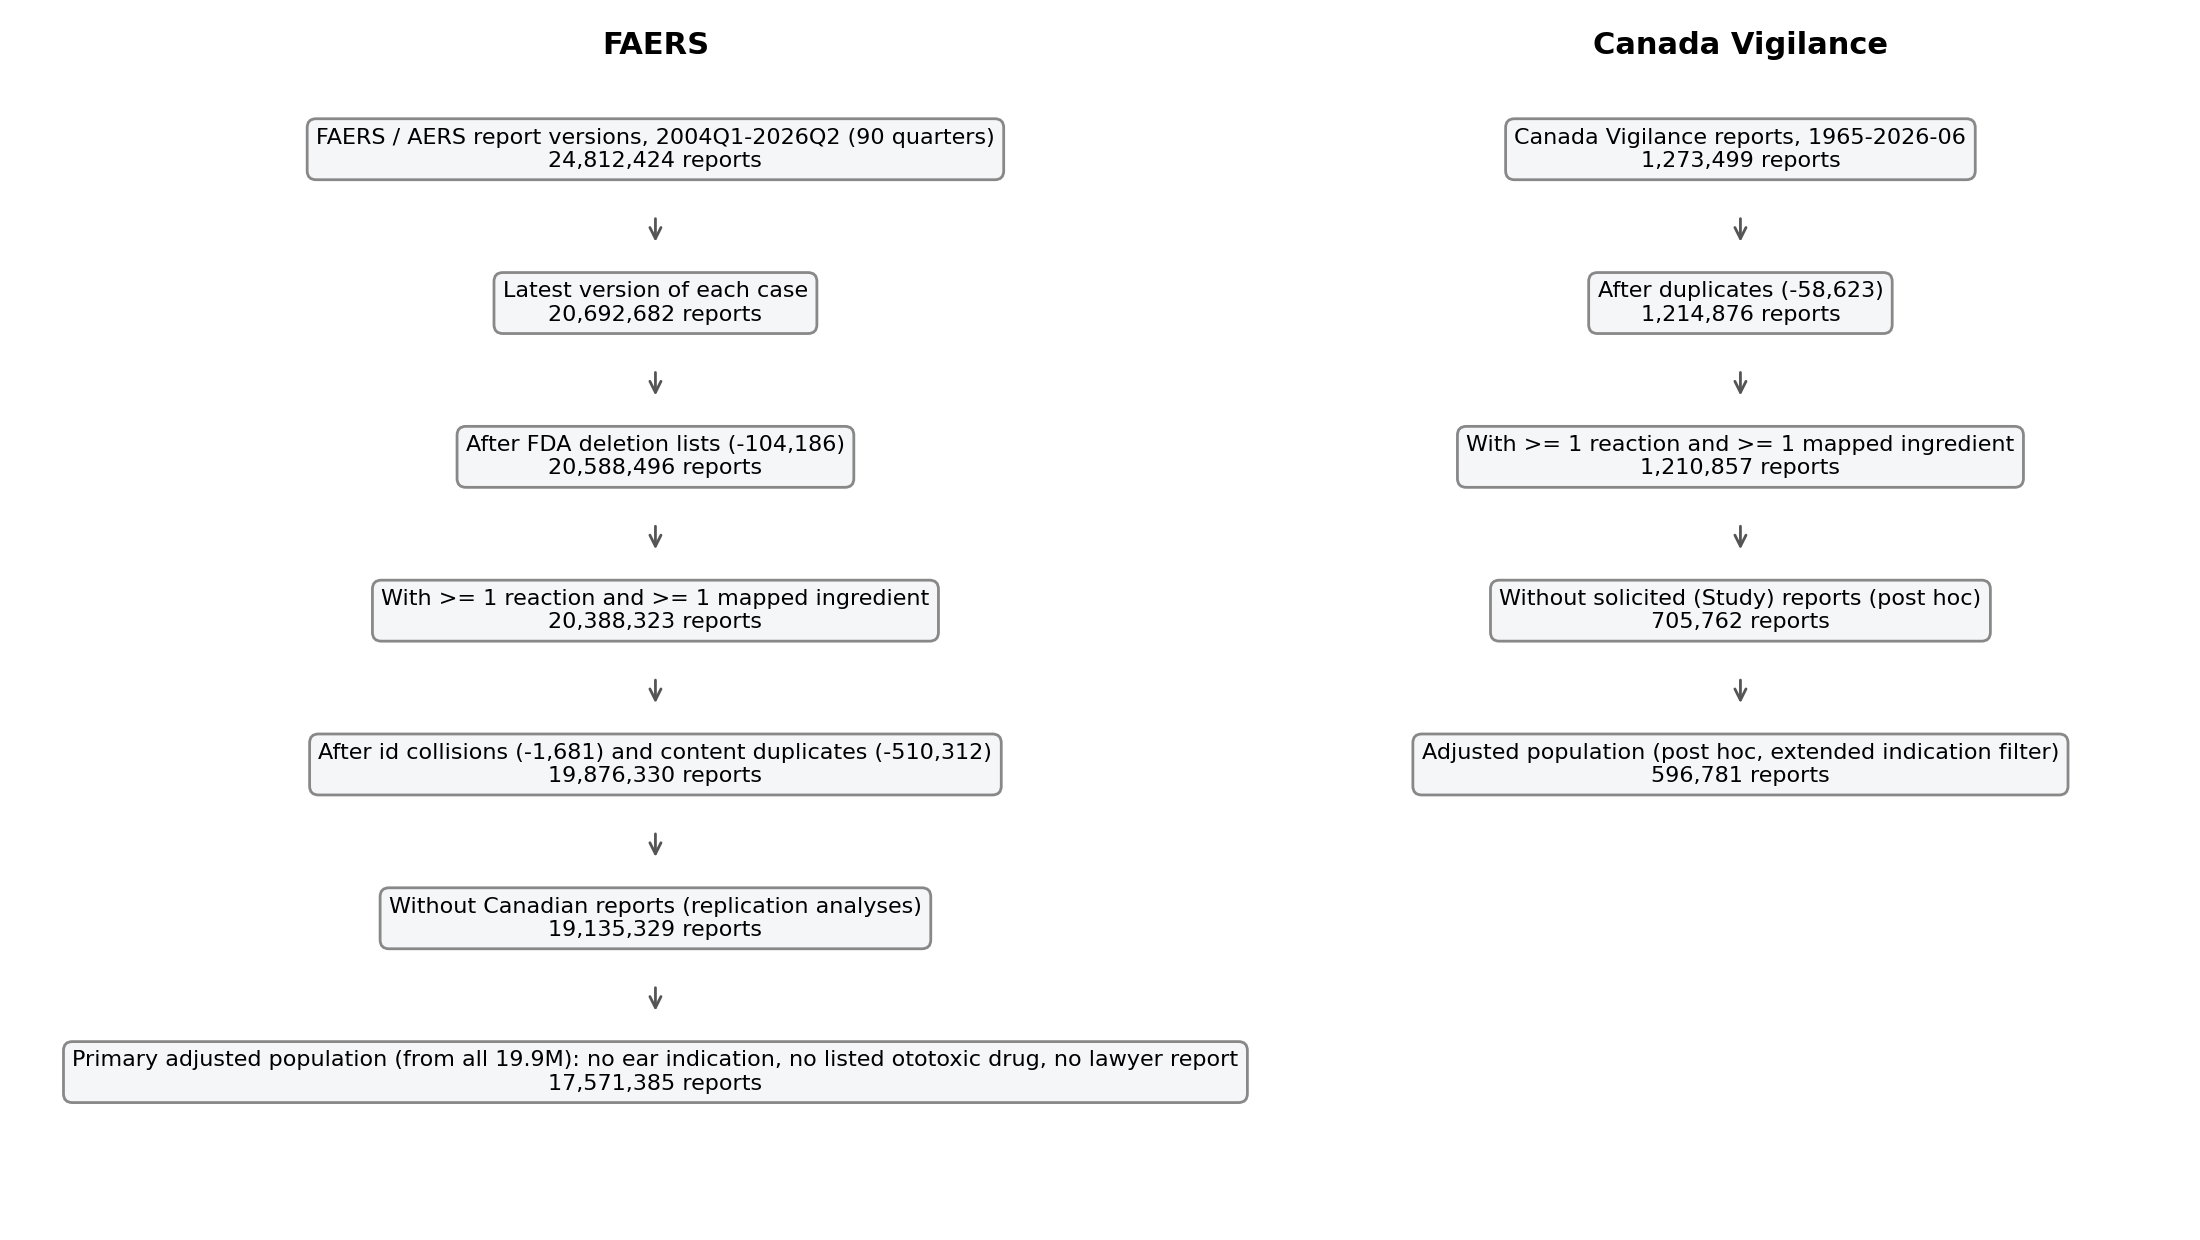
\includegraphics[width=\textwidth]{../figures/flow.png}

\section*{Table S3. Case-level review of robust signals absent from all US labels (post hoc)}
Rubric, first applicable category: K established ototoxic class or association documented by a prospective/cohort series;
A report cluster ($\geq$50\% of cases in reports listing $\geq$15 drugs); B $\geq$50\% of cases co-name an established ototoxic
drug; C stimulated or solicited reporting; D main indication associated with the event; E none. Cat.\,1: author; Cat.\,2:
second, AI-based assessor, blind to Cat.\,1, before the active-comparator rule (agreement 19/22, $\kappa=0.82$). Category D
also requires the active-comparator (within-indication) ROR lower bound $\leq 1$. Profiles: FAERS cases without Canadian reports.
{\footnotesize
\begin{longtable}{p{2.2cm}lccrllrrrrp{2.2cm}p{4.6cm}}
\toprule
Drug & Event & Cat.\,1 & Cat.\,2 & Cases & Top country & Top year & Consumer & Median drugs & $\geq$15 drugs & Ototoxic co-drug & Within-indication ROR & Note \\
\midrule
Rofecoxib & HL & C & C & 243 & US 64\% & 2006 42\% & 7\% & 6 & 14\% & 33\% &  & litigation-era reporting (2004-2006) \\
Tozinameran & HL & C & K & 57 & US 40\% & 2022 28\% & 72\% & 6 & 26\% & 5\% &  & mass vaccination; cohort evidence conflicting (Israel SIR 1.35, PMID 35201275; Denmark null, PMID 37288514) \\
Elasomeran & HL & C & C & 20 & US 85\% & 2023 35\% & 75\% & 8 & 35\% & 20\% &  & mass vaccination; media attention to hearing effects \\
Etanercept & HL & D & D & 2095 & US 80\% & 2016 20\% & 49\% & 1 & 3\% & 4\% & 0.93 (0.87-1.00) & rheumatoid arthritis associated with SNHL (PMID 32488430); used for autoimmune inner ear disease \\
Insulin Aspart & HL & D & D & 250 & US 85\% & 2025 17\% & 82\% & 2 & 5\% & 2\% & 1.17 (1.00-1.37) & diabetes associated with hearing impairment (meta-analysis, PMID 23150692) \\
Tofacitinib & HL & E & D & 1728 & US 94\% & 2022 19\% & 82\% & 1 & 4\% & 7\% & 2.24 (2.06-2.45) & persists against other RA drugs; 82 \% consumer reports; rheumatoid arthritis associated with SNHL (PMID 32488430) \\
Pregabalin & HL & E & E & 1703 & US 86\% & 2021 23\% & 62\% & 2 & 12\% & 11\% & 3.27 (3.04-3.52) & alpha-2-delta ligand; one case report of reversible loss (PMID 32297964); diabetes/neuropathy and age (median 71) confound; labels list tinnitus and hyperacusis, not hearing loss \\
Amlodipine & HL & E & D & 792 & US 29\% & 2021 15\% & 70\% & 4 & 9\% & 14\% & 1.89 (1.69-2.10) & labels list tinnitus; VA cohort found lower SNHL risk with calcium-channel blockers (PMID 34855682); hypertension associated with hearing loss (meta-analysis, PMID 39839866) \\
Glycopyrrolate & HL & E & D & 315 & US 75\% & 2025 27\% & 50\% & 3 & 3\% & 4\% & 1.65 (1.27-2.14) & persists against other COPD drugs; COPD associated with hearing loss (PMID 38828668) \\
Travoprost & HL & E & D & 140 & US 61\% & 2019 23\% & 75\% & 1 & 0\% & 3\% & 2.43 (1.80-3.29) & persists against other glaucoma drugs; median age 80; glaucoma associated with SNHL (PMID 31935130) \\
Candesartan & Tin & A & A & 422 & GB 80\% & 2023 54\% & 38\% & 42 & 83\% & 34\% &  & 83\% of cases in reports listing >= 15 drugs \\
Propranolol & Tin & A & A & 189 & PT 50\% & 2024 21\% & 24\% & 71 & 66\% & 66\% &  & 66\% of cases in reports listing >= 15 drugs \\
Tozinameran & Tin & A & A & 109 & GB 52\% & 2023 38\% & 46\% & 28 & 51\% & 48\% &  & 51\% of cases in reports listing >= 15 drugs; mass vaccination; cohort evidence conflicting (Israel SIR 1.35, PMID 35201275; Denmark null, PMID 37288514) \\
Indapamide & Tin & A & A & 44 & PL 50\% & 2018 23\% & 18\% & 15.5 & 55\% & 59\% &  & 55\% of cases in reports listing >= 15 drugs \\
Finasteride & Tin & C & C & 293 & GB 38\% & 2024 17\% & 60\% & 1 & 0\% & 1\% &  & post-finasteride syndrome advocacy reporting \\
Rofecoxib & Tin & C & C & 189 & US 58\% & 2006 47\% & 8\% & 6 & 21\% & 26\% &  & litigation-era reporting (2004-2006) \\
Elasomeran & Tin & C & C & 13 & US 54\% & 2023 38\% & 69\% & 8 & 31\% & 23\% &  & mass vaccination; media attention to hearing effects \\
Galcanezumab & Tin & D & E & 96 & US 94\% & 2020 28\% & 88\% & 1 & 0\% & 1\% & 0.82 (0.63-1.06) & migraine associated with tinnitus (systematic review, PMID 36459425; a meta-analysis found low evidence, PMID 36380120) \\
Chlorthalidone & Tin & D & E & 10 & US 70\% & 2025 20\% & 90\% & 4 & 0\% & 0\% & 1.04 (0.43-2.51) & hypertension associated with tinnitus (meta-analysis, PMID 26881064) \\
Doxycycline & Tin & E & E & 220 & US 43\% & 2024 13\% & 48\% & 3 & 6\% & 23\% & 3.63 (2.98-4.42) & pulsatile tinnitus can accompany labelled drug-induced intracranial hypertension (PMID 38516546), but only 15/220 cases co-report intracranial hypertension or papilloedema \\
Liothyronine & Tin & E & D & 40 & US 57\% & 2023 35\% & 78\% & 5.5 & 32\% & 2\% & 2.10 (1.31-3.36) & persists against other hypothyroidism drugs; 32 \% drug-dense reports (UK cluster overlap); hypothyroidism associated with tinnitus (PMID 35233053) \\
Paromomycin & Tin & K & K & 3 & US 67\% & 2017 33\% & 67\% & 1 & 0\% & 0\% &  & on the a-priori ototoxic list (aminoglycoside); oral aminoglycoside, poorly absorbed; 3 cases \\
\bottomrule
\end{longtable}}

\section*{Table S4. Characteristics of FAERS hearing-loss and tinnitus reports and all other reports (READUS-PV item 8b)}
The hearing-loss and tinnitus groups overlap: 6{,}722 reports contain both events and are counted in both columns.
``All other reports'' are reports with neither event, so the three columns sum to more than the 19{,}876{,}330 reports analysed.
\begin{longtable}{lrrr}
\toprule
 & Hearing loss & Tinnitus & All other reports \\
\midrule
Reports, n & 83,883 & 42,900 & 19,756,269 \\
Age, median (years) & 67 & 55 & 58 \\
\textit{Age} & & & \\
\quad <18 (\%) & 2.4 & 1.2 & 3.5 \\
\quad 18-44 (\%) & 6.9 & 16.3 & 12.5 \\
\quad 45-64 (\%) & 15.6 & 30.0 & 20.2 \\
\quad $\geq$65 (\%) & 30.6 & 17.4 & 20.7 \\
\quad unknown (\%) & 44.5 & 35.1 & 43.1 \\
\textit{Sex} & & & \\
\quad female (\%) & 52.9 & 58.3 & 52.7 \\
\quad male (\%) & 39.3 & 32.2 & 34.3 \\
\quad unknown (\%) & 7.8 & 9.5 & 13.0 \\
\textit{Reporter} & & & \\
\quad consumer (\%) & 60.0 & 53.7 & 44.2 \\
\quad physician (\%) & 16.2 & 16.9 & 21.6 \\
\quad pharmacist (\%) & 3.2 & 4.7 & 6.1 \\
\quad other health professional (\%) & 12.6 & 14.2 & 18.6 \\
\quad lawyer (\%) & 0.8 & 1.8 & 2.5 \\
\quad unknown (\%) & 7.2 & 8.7 & 6.9 \\
\textit{Country} & & & \\
\quad United States (\%) & 69.9 & 64.0 & 71.3 \\
\quad other (\%) & 28.6 & 32.8 & 27.0 \\
\quad unknown (\%) & 1.5 & 3.2 & 1.7 \\
\textit{FDA receipt} & & & \\
\quad 2004-2012 (\%) & 13.6 & 21.2 & 15.6 \\
\quad 2013-2018 (\%) & 30.7 & 34.0 & 31.8 \\
\quad 2019-2026 (\%) & 55.7 & 44.8 & 52.6 \\
\bottomrule
\end{longtable}

\section*{Table S5. All robust signals (post hoc: adjusted FAERS signal replicated adjusted-to-adjusted in Canada Vigilance without solicited reports)}
FAERS: adjusted MH OR (extended indication filter, Canadian reports excluded); Canada: adjusted MH OR; Label: event on any US label of a product containing the drug.
{\footnotesize
\begin{longtable}{lcrcrcc}
\toprule
Ingredient & Event & FAERS adj.\ cases & FAERS adj.\ OR (95\% CI) & Canada adj.\ cases & Canada adj.\ OR (95\% CI) & Label \\
\midrule
Amikacin & HL & 454 & 12.71 (11.55--13.98) & 20 & 286.54 (160.73--510.83) & yes \\
Amlodipine & HL & 675 & 2.39 (2.21--2.57) & 16 & 2.70 (1.65--4.44) & no \\
Amphotericin B & HL & 43 & 1.53 (1.14--2.07) & 3 & 6.30 (2.01--19.75) & yes \\
Azithromycin & HL & 404 & 5.15 (4.66--5.68) & 30 & 11.05 (7.65--15.96) & yes \\
Bupropion & HL & 219 & 1.15 (1.01--1.32) & 21 & 2.46 (1.59--3.80) & yes \\
Ciprofloxacin & HL & 400 & 2.94 (2.66--3.24) & 35 & 4.47 (3.19--6.27) & yes \\
Cisplatin & HL & 688 & 4.30 (3.98--4.64) & 47 & 20.99 (15.49--28.45) & yes \\
Clarithromycin & HL & 196 & 3.40 (2.95--3.91) & 21 & 5.45 (3.52--8.43) & yes \\
Deferasirox & HL & 290 & 4.02 (3.58--4.52) & 6 & 4.29 (1.91--9.66) & yes \\
Deferoxamine & HL & 35 & 9.60 (6.85--13.45) & 24 & 81.44 (51.89--127.82) & yes \\
Elasomeran & HL & 16 & 2.36 (1.44--3.86) & 16 & 3.30 (2.01--5.44) & no \\
Erythromycin & HL & 57 & 2.29 (1.76--2.97) & 20 & 7.74 (4.90--12.22) & yes \\
Etanercept & HL & 2003 & 1.15 (1.10--1.21) & 49 & 2.28 (1.71--3.05) & no \\
Ethacrynic Acid & HL & 4 & 13.94 (5.07--38.28) & 5 & 109.98 (41.12--294.17) & yes \\
Furosemide & HL & 209 & 1.19 (1.04--1.36) & 14 & 4.42 (2.59--7.53) & yes \\
Gentamicin & HL & 168 & 11.96 (10.24--13.97) & 90 & 65.05 (50.65--83.55) & yes \\
Glycopyrrolate & HL & 303 & 3.08 (2.74--3.45) & 5 & 4.40 (1.82--10.67) & no \\
Hydroxychloroquine & HL & 133 & 1.80 (1.51--2.13) & 63 & 2.03 (1.57--2.62) & yes \\
Insulin Aspart & HL & 243 & 2.27 (2.00--2.58) & 5 & 2.69 (1.11--6.50) & no \\
Moxifloxacin & HL & 132 & 2.12 (1.78--2.51) & 23 & 6.87 (4.52--10.43) & yes \\
Neomycin & HL & 52 & 4.97 (3.77--6.54) & 6 & 8.70 (3.85--19.66) & yes \\
Peginterferon Alfa-2B & HL & 64 & 1.54 (1.20--1.96) & 7 & 4.57 (2.15--9.70) & yes \\
Piroxicam & HL & 15 & 2.20 (1.32--3.65) & 3 & 5.65 (1.80--17.75) & yes \\
Pregabalin & HL & 1497 & 3.25 (3.09--3.43) & 15 & 2.06 (1.24--3.44) & no \\
Ramipril & HL & 82 & 1.27 (1.02--1.58) & 10 & 2.34 (1.25--4.37) & yes \\
Ribavirin & HL & 323 & 1.25 (1.12--1.40) & 11 & 1.98 (1.09--3.61) & yes \\
Rofecoxib & HL & 143 & 2.39 (2.02--2.82) & 10 & 4.42 (2.35--8.31) & no \\
Sildenafil & HL & 705 & 4.04 (3.74--4.35) & 23 & 5.44 (3.57--8.28) & yes \\
Streptomycin & HL & 12 & 9.18 (5.17--16.29) & 6 & 8.80 (3.89--19.93) & yes \\
Tadalafil & HL & 587 & 4.42 (4.07--4.79) & 17 & 4.43 (2.71--7.22) & yes \\
Terbinafine & HL & 99 & 3.29 (2.70--4.01) & 5 & 3.09 (1.28--7.48) & yes \\
Tobramycin & HL & 232 & 4.82 (4.23--5.49) & 17 & 23.12 (14.12--37.86) & yes \\
Tofacitinib & HL & 1608 & 3.27 (3.11--3.45) & 53 & 1.39 (1.05--1.84) & no \\
Tozinameran & HL & 46 & 2.36 (1.76--3.15) & 109 & 7.04 (5.70--8.69) & no \\
Travoprost & HL & 135 & 3.71 (3.13--4.40) & 3 & 4.96 (1.58--15.54) & no \\
Vancomycin & HL & 209 & 2.21 (1.93--2.54) & 42 & 12.16 (8.87--16.67) & yes \\
Acetazolamide & Tin & 12 & 2.96 (1.68--5.23) & 3 & 5.11 (1.63--16.07) & yes \\
Amikacin & Tin & 233 & 17.86 (15.66--20.37) & 3 & 21.25 (6.56--68.80) & yes \\
Amitriptyline & Tin & 72 & 1.68 (1.33--2.12) & 11 & 1.96 (1.08--3.56) & yes \\
Amlodipine & Tin & 445 & 3.06 (2.79--3.36) & 16 & 2.50 (1.52--4.10) & yes \\
Aspirin & Tin & 615 & 3.01 (2.78--3.26) & 118 & 7.51 (6.19--9.10) & yes \\
Atenolol & Tin & 83 & 2.91 (2.35--3.62) & 8 & 3.91 (1.94--7.88) & yes \\
Azithromycin & Tin & 257 & 5.76 (5.09--6.52) & 22 & 6.00 (3.92--9.19) & yes \\
Bisoprolol & Tin & 321 & 13.85 (12.39--15.49) & 4 & 3.29 (1.23--8.83) & yes \\
Bupropion & Tin & 1058 & 7.90 (7.42--8.41) & 59 & 4.51 (3.47--5.87) & yes \\
Buspirone Hydrochloride & Tin & 44 & 3.84 (2.85--5.16) & 4 & 8.70 (3.20--23.61) & yes \\
Candesartan & Tin & 277 & 11.72 (10.40--13.22) & 15 & 2.80 (1.68--4.68) & no \\
Celecoxib & Tin & 154 & 1.67 (1.42--1.95) & 20 & 1.70 (1.09--2.65) & yes \\
Chlorthalidone & Tin & 10 & 1.94 (1.04--3.62) & 4 & 4.57 (1.70--12.29) & no \\
Choline & Tin & 4 & 23.45 (8.56--64.21) & 4 & 3.98 (1.48--10.70) & yes \\
Ciprofloxacin & Tin & 969 & 12.72 (11.92--13.57) & 52 & 4.98 (3.77--6.58) & yes \\
Cisplatin & Tin & 233 & 2.33 (2.05--2.65) & 17 & 5.81 (3.58--9.43) & yes \\
Citalopram & Tin & 179 & 2.37 (2.05--2.75) & 12 & 1.77 (1.00--3.13) & yes \\
Clonazepam & Tin & 254 & 2.99 (2.64--3.38) & 16 & 3.58 (2.18--5.88) & yes \\
Cyclobenzaprine & Tin & 33 & 1.57 (1.12--2.22) & 4 & 2.96 (1.10--7.95) & yes \\
Desvenlafaxine & Tin & 226 & 4.74 (4.15--5.40) & 9 & 4.16 (2.14--8.06) & yes \\
Dexchlorpheniramine & Tin & 8 & 4.34 (2.16--8.71) & 5 & 2.80 (1.16--6.78) & yes \\
Diltiazem & Tin & 48 & 1.70 (1.28--2.26) & 11 & 4.05 (2.23--7.38) & yes \\
Doxycycline & Tin & 159 & 4.54 (3.88--5.31) & 7 & 2.36 (1.12--4.97) & no \\
Duloxetine & Tin & 1718 & 12.40 (11.80--13.04) & 32 & 4.16 (2.92--5.92) & yes \\
Elasomeran & Tin & 10 & 3.62 (1.94--6.74) & 21 & 3.50 (2.26--5.43) & no \\
Felodipine & Tin & 220 & 73.24 (63.47--84.52) & 3 & 5.34 (1.70--16.75) & yes \\
Finasteride & Tin & 286 & 9.73 (8.63--10.95) & 5 & 3.04 (1.26--7.37) & no \\
Gabapentin & Tin & 341 & 2.02 (1.82--2.25) & 25 & 4.21 (2.83--6.28) & yes \\
Galcanezumab & Tin & 94 & 1.86 (1.52--2.28) & 5 & 16.70 (6.73--41.48) & no \\
Gentamicin & Tin & 45 & 5.75 (4.28--7.72) & 23 & 8.48 (5.55--12.97) & yes \\
Ibuprofen & Tin & 289 & 1.51 (1.34--1.69) & 36 & 2.89 (2.07--4.04) & yes \\
Indapamide & Tin & 18 & 2.05 (1.29--3.26) & 6 & 3.44 (1.53--7.71) & no \\
Indomethacin & Tin & 15 & 2.54 (1.53--4.22) & 9 & 2.68 (1.39--5.20) & yes \\
Irbesartan & Tin & 73 & 3.15 (2.50--3.97) & 6 & 2.26 (1.01--5.07) & yes \\
Isotretinoin & Tin & 212 & 2.69 (2.35--3.08) & 10 & 3.17 (1.69--5.94) & yes \\
Lidocaine & Tin & 90 & 1.67 (1.35--2.05) & 12 & 2.85 (1.61--5.04) & yes \\
Liothyronine & Tin & 38 & 4.90 (3.56--6.75) & 3 & 16.73 (5.22--53.59) & no \\
Mefloquine & Tin & 85 & 27.80 (22.24--34.74) & 8 & 14.52 (7.08--29.79) & yes \\
Minocycline & Tin & 49 & 4.01 (3.02--5.31) & 7 & 3.49 (1.65--7.36) & yes \\
Moxifloxacin & Tin & 151 & 3.51 (2.99--4.13) & 21 & 4.65 (3.01--7.18) & yes \\
Naproxen & Tin & 445 & 3.05 (2.77--3.35) & 23 & 2.42 (1.60--3.66) & yes \\
Nifedipine & Tin & 24 & 1.51 (1.01--2.26) & 7 & 2.95 (1.40--6.22) & yes \\
Norfloxacin & Tin & 7 & 4.63 (2.19--9.75) & 4 & 6.03 (2.23--16.29) & yes \\
Nortriptyline & Tin & 29 & 2.80 (1.94--4.04) & 6 & 3.96 (1.76--8.87) & yes \\
Paromomycin & Tin & 3 & 27.75 (8.63--89.29) & 3 & 262.76 (53.09--1300.46) & no \\
Paroxetine & Tin & 478 & 5.19 (4.74--5.69) & 38 & 5.12 (3.70--7.11) & yes \\
Penicillin G Procaine & Tin & 5 & 7.93 (3.27--19.22) & 5 & 10.12 (4.12--24.86) & yes \\
Perindopril Erbumine & Tin & 6 & 2.33 (1.05--5.20) & 12 & 3.59 (2.02--6.37) & yes \\
Propranolol & Tin & 65 & 1.79 (1.40--2.28) & 6 & 2.31 (1.03--5.17) & no \\
Quinine & Tin & 35 & 7.11 (5.09--9.94) & 10 & 23.00 (11.99--44.15) & yes \\
Rofecoxib & Tin & 131 & 2.53 (2.13--3.02) & 8 & 2.26 (1.12--4.54) & no \\
Sildenafil & Tin & 214 & 2.28 (1.99--2.61) & 12 & 2.59 (1.46--4.59) & yes \\
Streptomycin & Tin & 3 & 3.37 (1.08--10.51) & 14 & 10.88 (6.31--18.74) & yes \\
Telmisartan & Tin & 58 & 3.22 (2.49--4.17) & 8 & 2.02 (1.00--4.07) & yes \\
Terbinafine & Tin & 58 & 2.95 (2.28--3.82) & 7 & 2.87 (1.36--6.07) & yes \\
Tobramycin & Tin & 144 & 6.04 (5.12--7.12) & 7 & 6.50 (3.06--13.80) & yes \\
Topiramate & Tin & 193 & 2.68 (2.32--3.09) & 9 & 1.99 (1.03--3.84) & yes \\
Tozinameran & Tin & 56 & 6.53 (5.01--8.50) & 171 & 10.11 (8.46--12.07) & no \\
Tramadol & Tin & 183 & 1.46 (1.26--1.69) & 10 & 1.99 (1.07--3.72) & yes \\
Trazodone Hydrochloride & Tin & 59 & 1.33 (1.03--1.72) & 12 & 4.63 (2.61--8.20) & yes \\
Valsartan & Tin & 347 & 1.43 (1.29--1.59) & 14 & 2.23 (1.31--3.80) & yes \\
Vancomycin & Tin & 90 & 1.68 (1.37--2.07) & 9 & 2.03 (1.05--3.92) & yes \\
Venlafaxine Hydrochloride & Tin & 603 & 4.96 (4.57--5.38) & 6 & 3.15 (1.40--7.05) & yes \\
Vortioxetine & Tin & 84 & 2.74 (2.21--3.40) & 4 & 3.06 (1.14--8.20) & yes \\
\bottomrule
\end{longtable}}

\section*{Table S6. Signals of previous screens available only from abstracts}
\begin{longtable}{llrrrrrp{6cm}}
\toprule
Study & Scope & Reported & Crude & Adjusted & Replicated & Robust & Robust drugs \\
\midrule
narasimhaswamy2026 & tinnitus & 4 & 0 & 0 & 0 & 0 &  \\
narasimhaswamy2026 & tinnitus & 3 & 2 & 1 & 1 & 1 & IBUPROFEN \\
wang2024 & tinnitus & 3 & 2 & 2 & 2 & 2 & CIPROFLOXACIN;DULOXETINE \\
wu2025 & hearing\_loss & 5 & 3 & 2 & 0 & 0 &  \\
\bottomrule
\end{longtable}
\end{document}
